\documentclass[aspectratio=169]{beamer}

% Language setup
\usepackage[magyar]{babel} % Babel for Hungarian
\usepackage[T1]{fontenc} % Output character encoding
\usepackage[utf8]{inputenc} % Input character encoding
\selectlanguage{magyar}

% Beamer styling setup
\usetheme{Boadilla}
\usecolortheme{default}
%\setbeamercolor{titlelike}{parent=structure,bg=gray!15}
\setbeamertemplate{navigation symbols}{}
\setbeamertemplate{caption}[numbered]
%

% Spacing setup
\setlength{\parindent}{0pt} % No paragraph indenting
\setlength{\parskip}{5pt} % Set spacing between paragraphs
\frenchspacing
\newcommand{\mkspace}{\vspace{19pt}}
\newcommand{\rmspace}{\vspace{-19pt}}
\newcommand{\emptyline}{\vspace{\baselineskip}}
%

% Dependency setup
\usepackage{tikz}
\usetikzlibrary{decorations.markings}
\usetikzlibrary{calc}
%

% Style setup
\usepackage{caption}
\captionsetup{format=plain, font=scriptsize, labelformat=empty}
%


% Notation setup
\usepackage{physics} % Braket notation

\author{Nemkin Viktória}
\title{Kvantum gráfbolyongások}
\date{}

\begin{document}

\frame{\titlepage}

\begin{frame}
  \frametitle{Kvantum gráfbolyongások}
  \textbf{Gráfbolyongások}
  \begin{itemize}
    \item Irányított, élsúlyozott gráf
    \item Csúcsokon lépkedés
    \item Kimenő élek súlya
  \end{itemize}

\end{frame}

\begin{frame}
  \frametitle{Kvantumérme}

  \begin{center}
    \begin{tikzpicture}[scale=2]
      \coordinate (A) at (0,2);
      \coordinate (B1) at (-1,1);
      \coordinate (B2) at (1,1);
      \coordinate (C11) at (-1.5,0);
      \coordinate (C12) at (-0.5,0);
      \coordinate (C21) at (0.5,0);
      \coordinate (C22) at (1.5,0);
      \begin{scope}[
          thin,
          decoration={
              markings,
              mark=at position 0.7 with {\arrow[scale=2]{>}}
            }
        ]
        \draw[thin, postaction={decorate}] (A) -- (B1);
        \draw[thin, postaction={decorate}] (A) -- (B2);
        \draw[thin, postaction={decorate}] (B1) -- (C11);
        \draw[thin, postaction={decorate}] (B1) -- (C12);
        \draw[thin, postaction={decorate}] (B2) -- (C21);
        \draw[thin, postaction={decorate}] (B2) -- (C22);
      \end{scope}
      \node at (-0.7,1.65) {$\frac{1}{\sqrt{2}}$};
      \draw[draw=white, fill=white] (A) circle (0.2) node {$\ket{1}$};
      \draw[draw=white, fill=white] (B1) circle (0.2) node {$\ket{0}$};
      \draw[draw=white, fill=white] (B2) circle (0.2) node {$\ket{1}$};
      \draw[draw=white, fill=white] (C11) circle (0.2) node {$\ket{0}$};
      \draw[draw=white, fill=white] (C12) circle (0.2) node {$\ket{1}$};
      \draw[draw=white, fill=white] (C21) circle (0.2) node {$\ket{1}$};
      \draw[draw=white, fill=white] (C22) circle (0.2) node {$\ket{0}$};
    \end{tikzpicture}
  \end{center}

\end{frame}

\begin{frame}
  \frametitle{Egyenesen bolyongás}
  \begin{figure}[H]
    \centering
    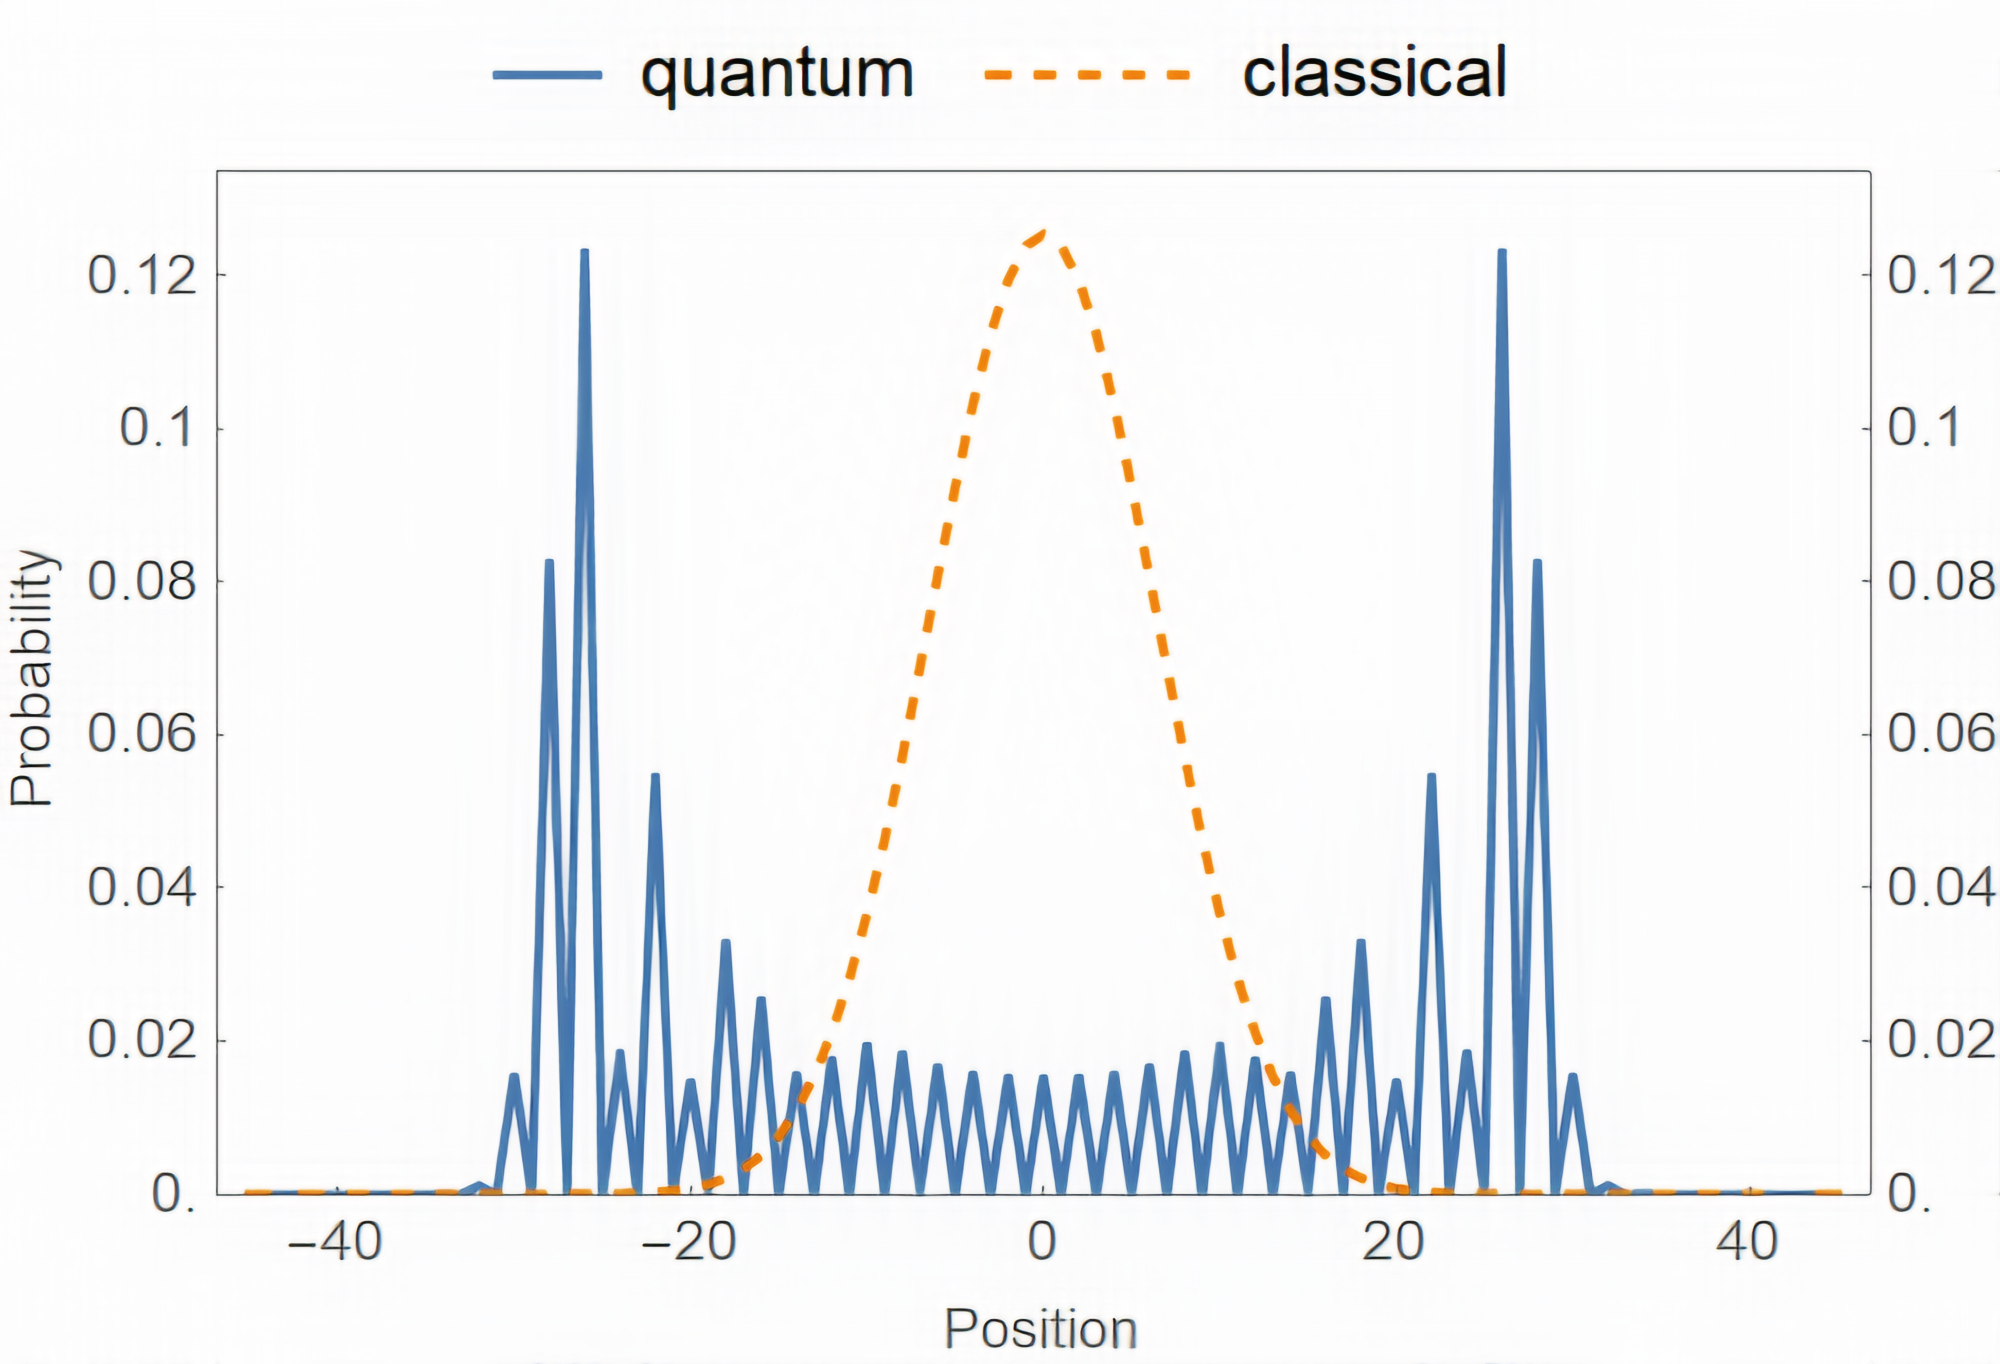
\includegraphics[width=0.6\linewidth]{./figures/teve.png}
  \end{figure}
\end{frame}

\begin{frame}
  \frametitle{Szimuláció: Egyenesen bolyongás}

  \begin{columns}[onlytextwidth]
    \begin{column}{.5\textwidth}
      \begin{figure}
        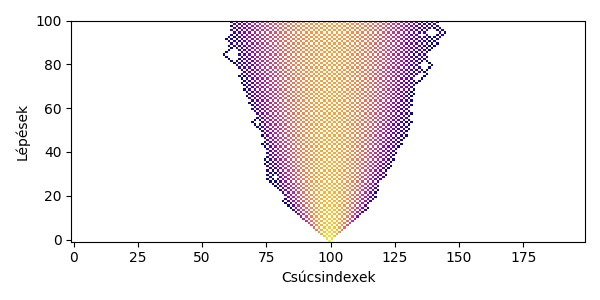
\includegraphics[width=\textwidth]{./figures/classical_simulation_short.jpg}
        \caption{\hspace{0.71cm}Klasszikus bolyongás}
      \end{figure}
    \end{column}
    \hfill
    \begin{column}{.5\textwidth}
      \begin{figure}
        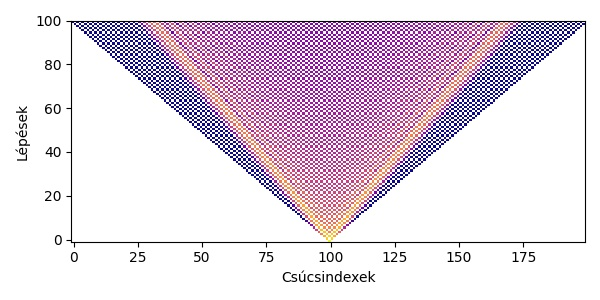
\includegraphics[width=\textwidth]{./figures/quantum_simulation_short.jpg}
        \caption{\hspace{0.73cm}Kvantum bolyongás}
      \end{figure}
    \end{column}
  \end{columns}
\end{frame}


\begin{frame}
  \frametitle{Szimuláció: Szakaszon bolyongás}

  \begin{columns}[onlytextwidth]
    \begin{column}{.25\textwidth}
    \end{column}
    \begin{column}{.25\textwidth}
      \begin{figure}
        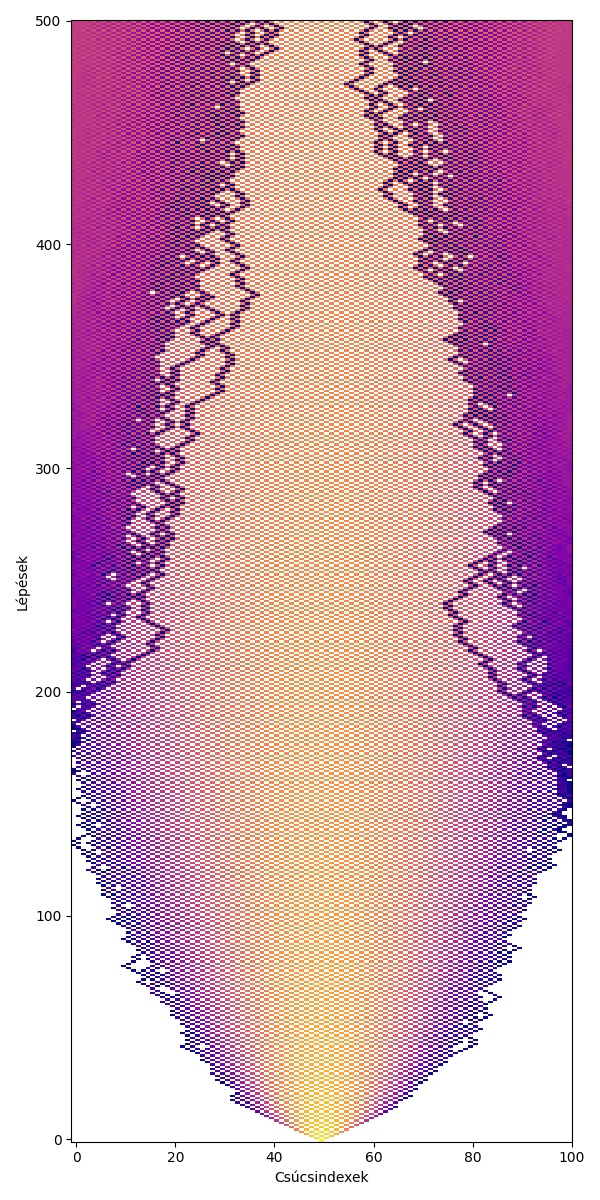
\includegraphics[width=0.9\textwidth]{./figures/classical_simulation_long.jpg}
        \caption{\hspace{0.28cm}Klasszikus bolyongás}
      \end{figure}
    \end{column}
    \begin{column}{.25\textwidth}
      \begin{figure}
        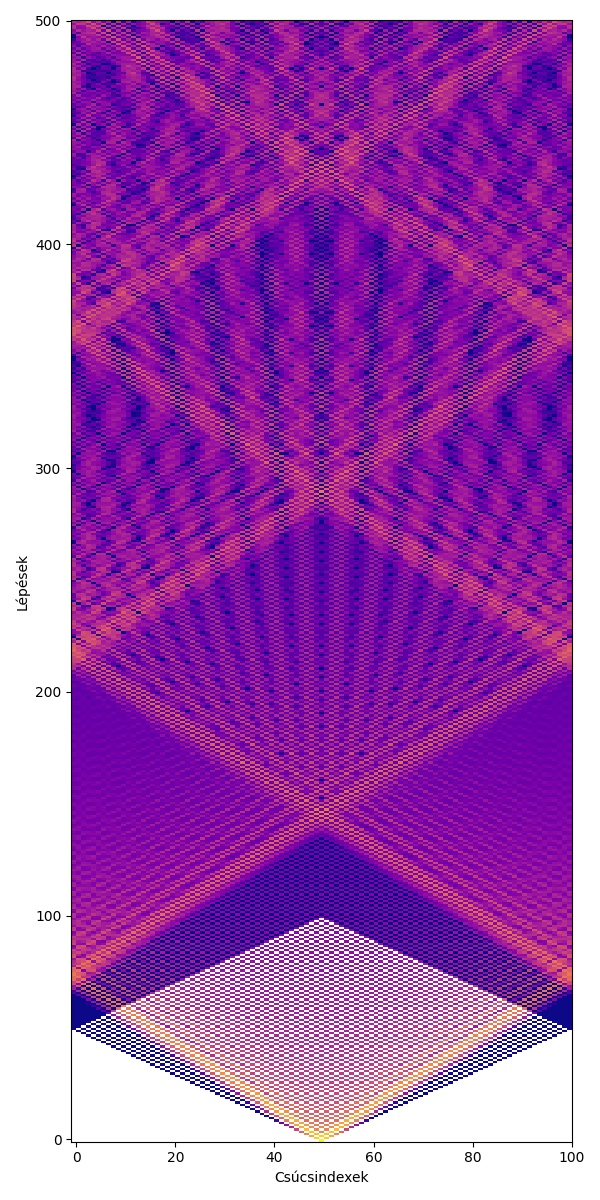
\includegraphics[width=0.9\textwidth]{./figures/quantum_simulation_long.jpg}
        \caption{\hspace{0.28cm}Kvantum bolyongás}
      \end{figure}
    \end{column}
    \begin{column}{.25\textwidth}
    \end{column}
  \end{columns}
\end{frame}


\end{document}
